\chapter[Results]{Results}
\label{sec:results}

This chapter explains the results obtained so far with the project development.


\section{Template for Games}
\label{sec:template_for_games}

The main goal of this work was to generate a template that allowed the game developers from the courses of this University to create their games and easily generate packages to install in major Operating Systems, namely, Windows, macOS, Debian-based and Red Hat based distributions of GNU/Linux. This template was made by professor Edson and I had the responsibility of evolving, maintaining and testing it in a few games, throughout all the platforms.

The template supports creating two versions of the executable: \texttt{debug}, that is supposed to be used on the development environment; and \texttt{release}, that is compiled with optimization flags and is supposed to be sent in packages to the users. It also has support for the most common SDL libraries used in game developing, like SDL, SDL\_image, SDL\_mixer. Each of these libraries is available for all the platforms, with the specifics for each inside of them.


\section{Platform}
\label {sec:platform}

The team developing this first version of the platform was able to integrate Django and React with some difficulty. Both of the technologies chosen are very well established on their own. Putting them together, however, is another matter, where they had a real hard time to make everything work right. They used React as the main user interface and Django Admin package to create the administrator part of the game.

The website as of now allows an administrator to upload a game, with its respective information, like supported platform, related media, and installers.
The administrator has to manually add all the information related to a game, like developers who worked on it, awards won (if any), release date, version number, etc. Figure \ref{fig:include_game1} shows part of the screen to add a game.

\begin{figure}[h!]
\centering
\fbox{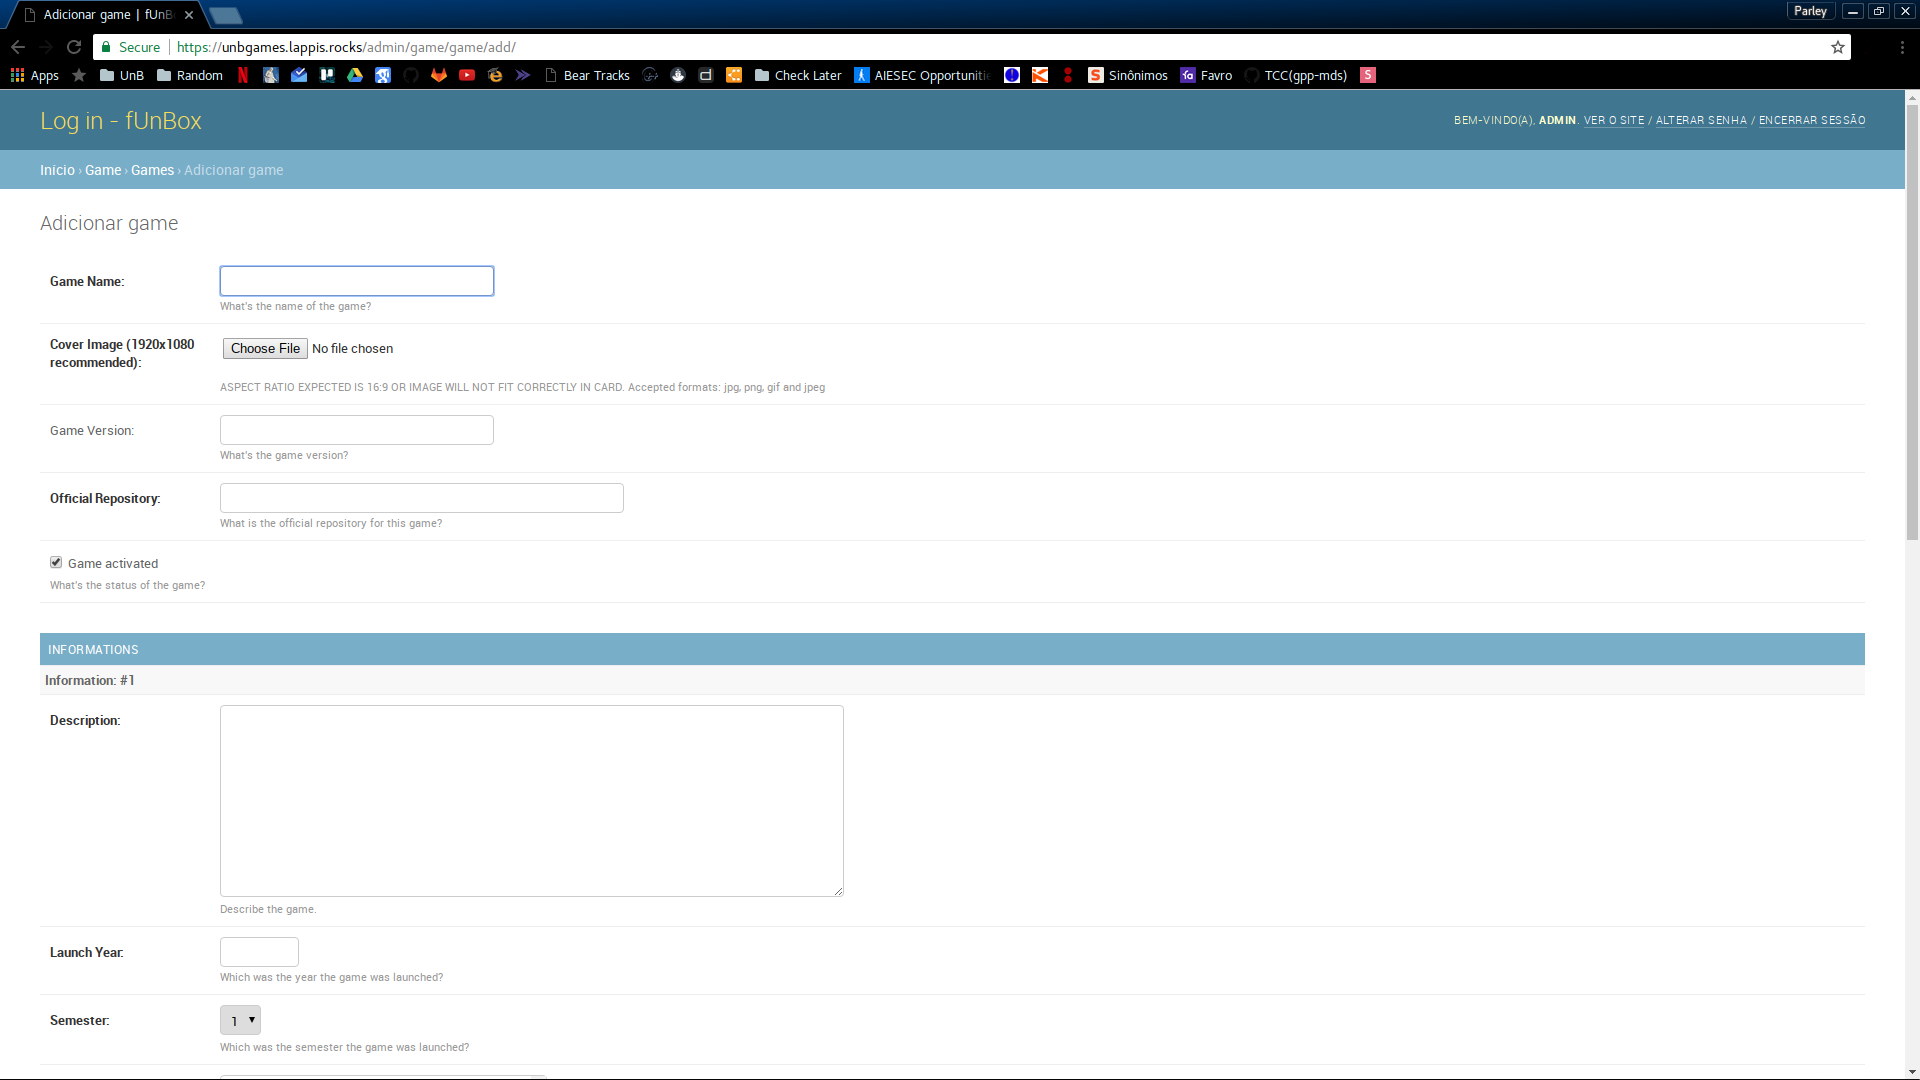
\includegraphics[width=\textwidth,height=\textheight,keepaspectratio]{include_game1}}
\caption{Include new game}
\label {fig:include_game1}
\end{figure}

The general public can see a list of the available games, with their uploaded pictures. The home page also shows a slide with some pictures of highlighted games. By choosing one, it's possible to see its version, official repository, release date, description, among other information.

Some other features of the platform are the possibility to download the game for the available operating systems or comment using a Facebook account, as shown in Figure \ref{fig:game_detail}. It's also possible to categorize the games and apply several filters on them. The user can search for a specific game by its name or description as well.

The team reported they had some problems in their inner communication on this first part of the project. They are 13 people, while 5 were the managers and 8 were developers. For people without any experience in managing and with a very detailed and demanding process, like RUP, they said it was hard to balance everything.

They also said that the transition from one process to the other was a little hard, especially the role change, holding the meetings and making sure Scrum/XP were being followed correctly. The communication problem they had on the first part was mitigated in this second part of the semester, but their main difficulty now was scoring the User Stories.

They declared that, beyond all the struggling that has been detailed above, they were too naive to choose React and Django for the development of the platform. This integration is not something very trivial for experienced programmers in both frameworks, it was even harder for developers that didn't have any experience with any of them. They said it was hard to manage everything that had to be done, learn the new technologies and still merge them together.


\begin{figure}[h!]
\centering
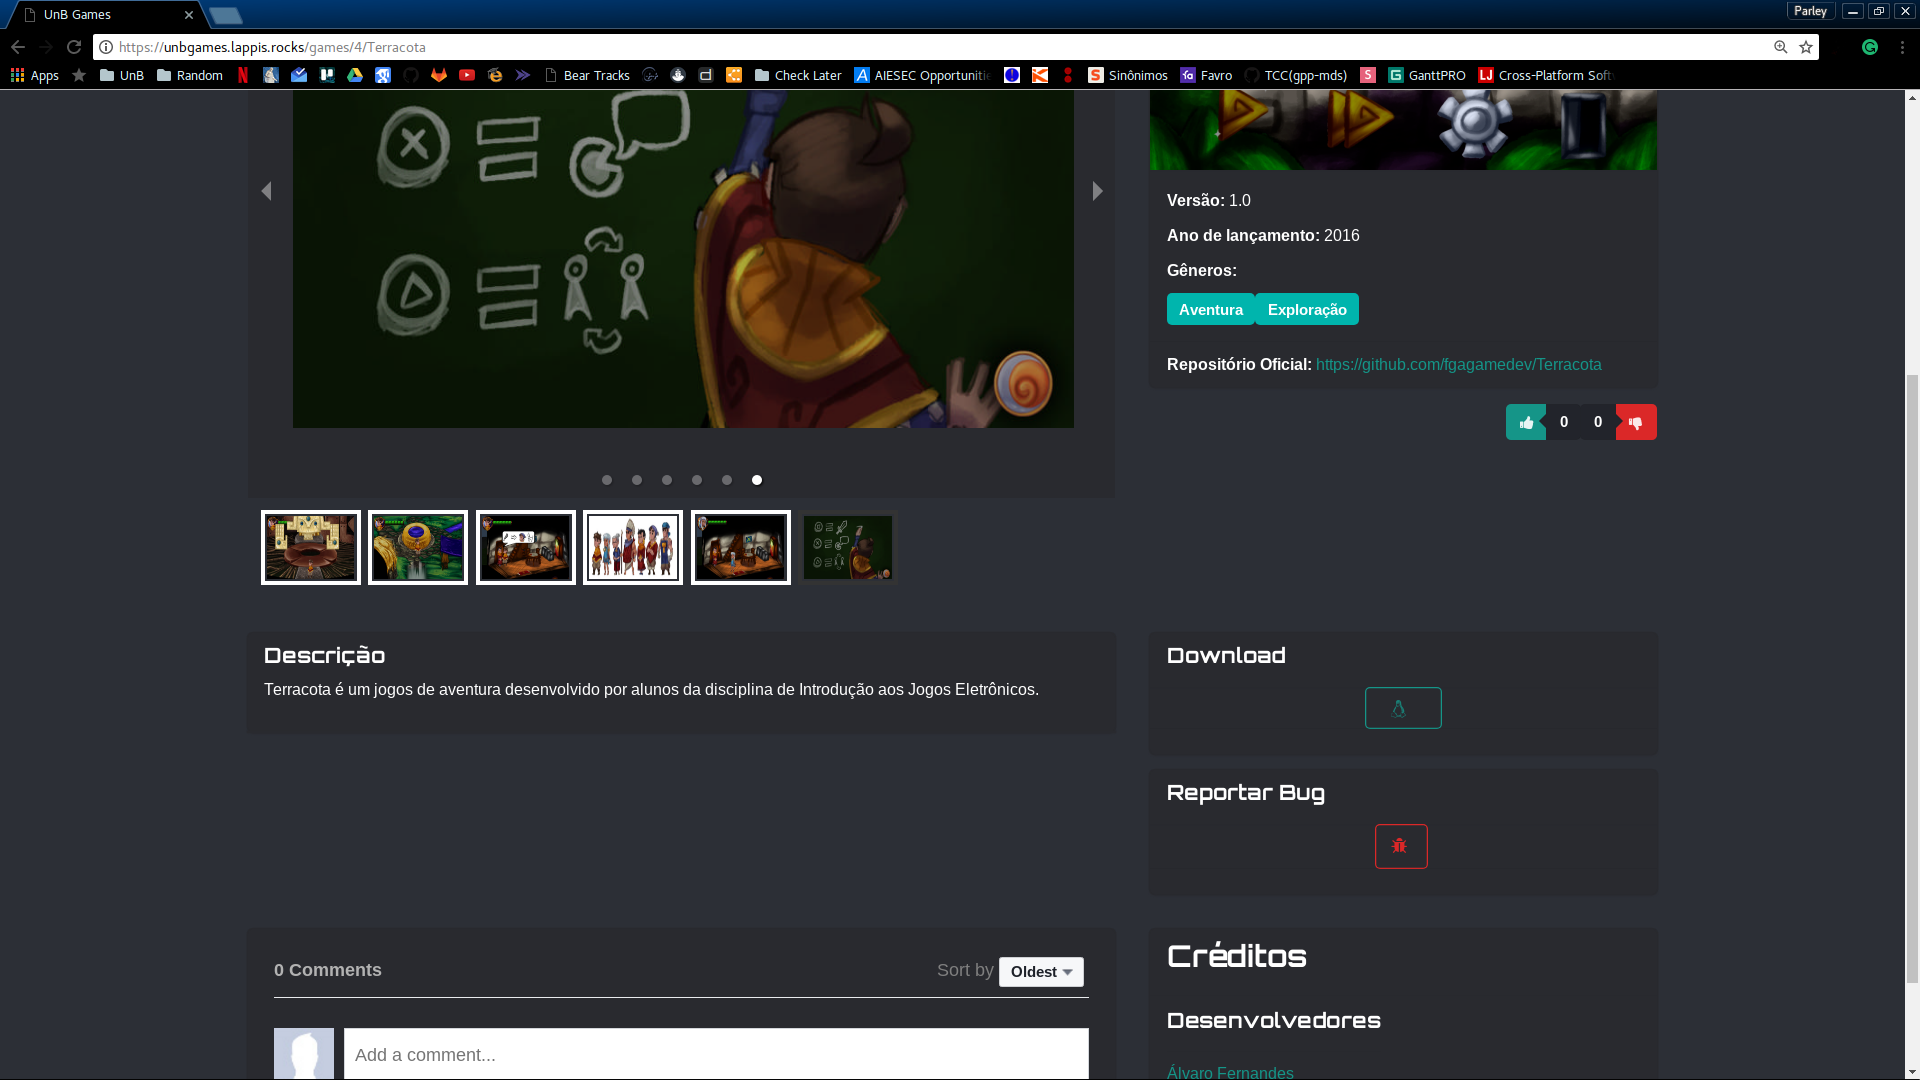
\includegraphics[width=\textwidth,height=\textheight,keepaspectratio]{terracota_detail}
\caption{Game detail}
\label {fig:game_detail}
\end{figure}

\section{Known Issues}
\label {sec:issues}

The building scripts have a few problems that will be fixed in the second part of the project:

\begin{itemize}
\item choosing a destination folder different than the user's home directory causes the Qt installer to fail. This is likely happening because somewhere on the Qt templates the symbol $\sim$ (abbreviation for home) is being used;

\item when the installation works successfully, the game doesn't run properly (or at all) on some systems (tested on Arch Linux for now). Probably there are some missing libraries on the final package, but this is just a hunch and has to be proved;

\item the games are running without sound, even on host systems that have full access to the sound card.
\end{itemize}

The platform also has a few issues that weren't resolved due to lack of time of the team. Some of them are described below:

\begin{itemize}
\item when an administrator tries to save a game without one or more needed fields an error occur, but all data is lost, requiring them to reenter all the information they had already typed. This may be happening because in the form validation, the team might be sending a new instance of the object instead of the one with the validation errors;

\item images are being saved multiple times when filling different forms (of the same game). They think this may happen because they retrieve and save all forms instead of just one with the images;

\item kernel choice is hard coded on the system;

\item when reporting a bug, the request breaks on some web browsers, like Chrome. They think it must be something with the protocol being used (HTTPS, for Chrome, and HTTP for Firefox).
\end{itemize}
